\documentclass[a4paper,12pt,final]{article}


\usepackage{graphicx}
\title{
\begin{center}
  	
\includegraphics[scale=0.3]{101Logo.png} 
  \end{center}
  \textbf{\\}
CSIR - Distributed Application Manager\\
Architectural Requirements Document\\
}
\author{101 Solutions}

\begin{document}
\maketitle
\begin{center}
Version 1.3
\end{center}
\textbf{\\}
\textbf{\\}
\textbf{\\}
\textbf{\\}
\textbf{\\}
\textbf{\\}
\begin{center}
\begin{tabular}{|l|l|}
\hline
Francois Germishuizen & 11093618\\
\hline
Jaco Swanepoel & 11016354\\
\hline
Henko van Koesveld & 11009315\\
\hline
\end{tabular}
\end{center}
\thispagestyle{empty}
\newpage
\thispagestyle{empty}
\textbf{\large{Change Log}}
\vspace{6pt}\newline
\begin{tabular}{|l|l|l|}
\hline
Date & Version & Description\\
\hline
13 Jun & Version 0.1 & Document Created\\
\hline
23 Jun & Version 0.2 & Added section 1.4 and 4\\
\hline
25 Jun & Version 0.3 & Added versioning system\\
\hline
25 Jun & Version 0.4 & Added initial section 2 and 6\\
\hline
26 Jun & Version 0.5 & Completed section 1.2\\
\hline
27 Jun & Version 0.6 & Completed section 3\\
\hline
28 Jun & Version 0.7 & Completed section 1.3 and 5\\
\hline
28 Jun & Version 0.8 & Proofread and added some content\\
\hline
28 Jun & Version 0.9 & Added glossary section\\
\hline
28 Jun & Version 1.0 & Final grammar and spelling check\\
\hline
11 Sep & Version 1.1 & Added changes as specified\\
\hline
12 Sep & Version 1.2 & Added few changes\\
\hline
15 Sep & Version 1.3 & Final grammar and spelling check\\
\hline
\end{tabular}
\newpage
\tableofcontents
\thispagestyle{empty}
\newpage

\pagenumbering{arabic}
\section{Overview}
\subsection{Background}
The CSIR is actively developing a distributed simulation framework that ties
in with various other real systems and is used to exchange information
between them. The client has a number of configurations of this system
depending on the requirements of the client which can involve various
external applications as well.\\
\textbf{\\}
One of the issues the client has is to quickly distribute the latest build or
configuration files of their software over various computers that are needed
for an experiment. In some cases the same computers may be used for other
experiments which mean each of the computers may need to have various
builds and configuration options.\\
\textbf{\\}
Another issue they experience is the running, stopping and restarting of
the complete simulation. During a simulation it may be determined that
certain configuration options may need to be changed and distributed to the
affected machines, in which case either all or some components will need to
be restarted which can become tedious and time consuming.
\subsection{Business opportunity}
The goal of our project is to develop an application which is able to maintain
various build versions of the simulation framework and distribute these builds
to certain designated machines that may be required for an experiment. The
application will monitor system statistics of the various machines attached
to an experiment and will have the ability to execute applications on those
machines which will have different configuration options.\\
\textbf{\\}
The application will consist of a master and slave component where the
master is used to control the distribution of slaves. From the master one will
be able to start an experiment which will run the relevant applications on all
the necessary machines.


%\subsection{Vision}
%For this project we will make an application that will help the client manage
%their simulation framework that works over a network. Our core focus will be
%sending applications across the network, executing them and stopping them.
%We will also be monitoring the status of the slaves connected to this network
%to help the client decide which slaves they will use to run their simulations.

\newpage
\section{Architectural Scope/Responsibilities}
\begin{itemize}
\item Persistence is required when we add builds, slaves and simulations.
\item Integration will be done in a message based manner by passing JSON strings between the Masters and Slaves.
\end{itemize}
%Use the Architectural Scope section to discuss the architectural responsibilities of your system. These architectural responsibilities will later be assigned to the dierent architectural components. Examples of architectural responsibilities for your software system include persistence, integrate with DB, integrate with web user


\section{Quality Requirements}
\begin{itemize}
  \item \textbf{Installability} - The software should be able to easily install.
\item \textbf{Portability} - The software must run on both Windows and Linux without the need for further adjustments or 3rd party applications.
\item \textbf{Performance} - The software should be able to run optimally. Specifically when copying required build files, for example one large file will copy faster than many small files.
\item \textbf{Usability} - The software should be easy to use without the need to read extensive documentation on how to operate it.
\item \textbf{Look and feel} - Look and feel ties in with usabilty. How the software looks should conform to how it will be used, which should be in a visually intuitive manner.
\item \textbf{Reusability} - The software should be able to be reused within different contexts, while still fulfilling the necessary functional requirements.
\item \textbf{Reliability} - The software should be reliable to ensure that when build versions are updated all the required files are sent and received without failures occurring.
\end{itemize}


\newpage
\section{Access and integration channels}
\subsection{Master GUI}
Below is a screenshot the Master GUI. The different slave builds will each have a colour to indicate status. A Build can be clicked on the list and placed on the slave if and when it is required. This will initiate the copying sequence. Next a simulation is chosen and can be run on the simulation tab. As specified by our client, the simulations are the primary display.
\begin{center}
  	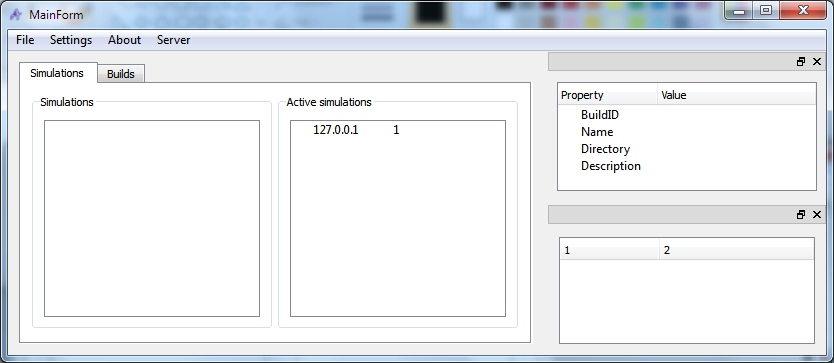
\includegraphics[scale=0.6]{AppManGuiSimPage.png}
 \end{center}
\begin{center}
  	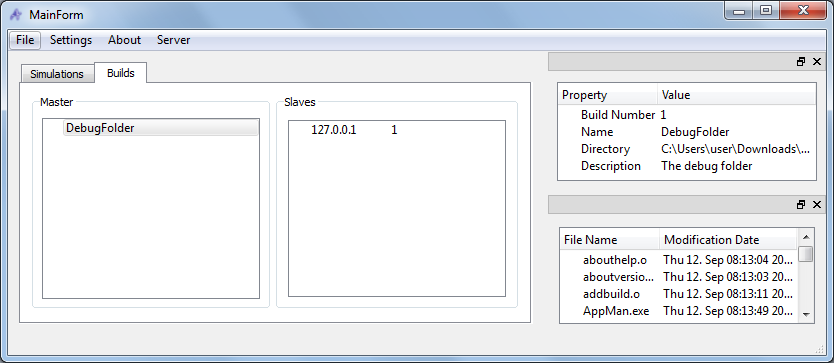
\includegraphics[scale=0.6]{AppManGuiBuildPage.png}
 \end{center}
 \newpage
 \subsection{Slave GUI}
Below is a screenshot of the Slave GUI. Builds can be viewed, added client side, system info can be requested and one can connect or disconnect from the master at the specified port.
\begin{center}
  	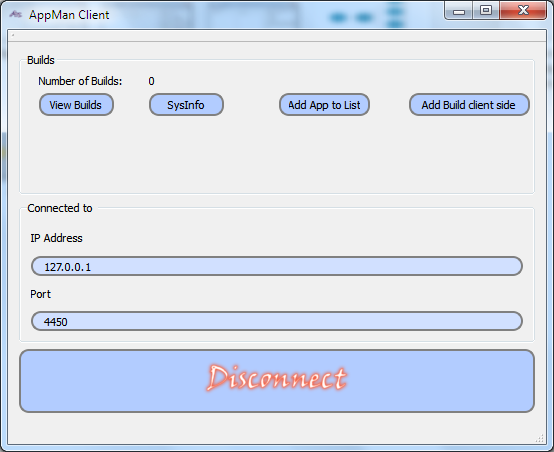
\includegraphics[scale=0.6]{AppManClientGui.png}
  \end{center} 
\subsection{Integration channels}
Below are the various channels we will be using:
\begin{itemize}
\item Connector/C++ 1.1.3 is available to connect to MySql for both Windows and Linux. It lets you develop C++ applications that connect to the MySQL Server.
\item XML parsing and handling will be done with the QXMLReader and QXMLWriter libraries used in our own classes for our needs.
\item QTcpSockets and c++ sockets from sys/socket.h are used to make a reliable connection between the Master and Slaves.
\end{itemize}
%pdflatex Architectural\ Requirements\ Document.tex
\newpage
\section{Architectural Constraints}
Overall constraints include the use of QT 4.8.4 with C++ throughout the project, as explicitly specified by the client.\\\textbf{\\}
The use of other technologies are allowed if need be such as 7zip for zipping and/or unzipping of files, however QT API's such as the file handling API must preferrably be used due to cross platform compiling.\\\textbf{\\}
Furthermore the project must be deployable on Windows and Linux and be capable of working on each of them.\\\textbf{\\}
For phase 2 in the project, the project must be capable of running applications on the slave computers that have been distributed from a master computer to a slave.\\\textbf{\\}
The configuration for the application to be run should also be used when running the program so that different environments can be selected. This is done with the creation of simulations.

\section{Patterns}
The project will make use of a Component based system combined with a Client server architecture. This is because the project needs the division of functionality for copying files, network, database and more.
\subsection{Component based system}
A Component based system is suitable as we have various concerns/components, such as a GUI to link to the management facade, a Server component, Slave component, Build component and Simulation component. The components fit together as follows:
\begin{center}
  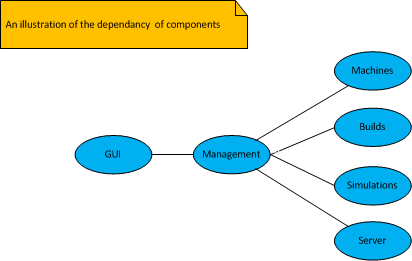
\includegraphics[scale=1]{ArchComponentDiag.png}
\end{center}
\subsection{Client server}
Client can in this case be the Master Computer or the Slave Computer. The server could potentially be in the Master or in the Slave, depending on the situation.
\begin{center}
  	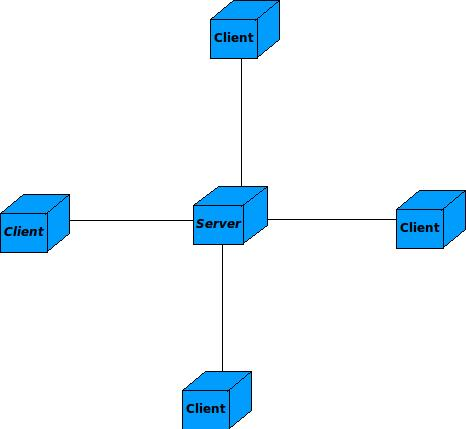
\includegraphics[scale=0.6]{ClientServer.jpeg} 
\end{center}

\newpage
\section{Architectural tactics or strategies}
\begin{itemize}
\item \textbf{Installability} - Using the QT framework, which allows source code to be built for various platforms, the software should be able to install on those platforms.
\item \textbf{Portability} - Using the QT framework, which allows source code to be built for various platforms, the software should be able to work on both Windows and Linux. Through use of "\#ifdef" statements in the source code we can also split Windows and Linux specific implementations.
\item \textbf{Performance} - Compiling and copying larger files will be quicker than copying a lot of small files. Using 7zip to compress small files will increase performance.
\item \textbf{Usability} - Using simple design and tooltips will allow for easy understanding of how the software is supposed to be used. A quick help section will also enhance understanding and usability.
\item \textbf{Look and feel} - Usabilty should also be enhanced by a visual intuitive layout that makes sense, is very simple and does not require typing. A simple drag and drop feature will be used to achieve this.
\item \textbf{Reusability} - The saving of configuations will allow the software to easily be reused to recreate simulations that have been run before.
\item \textbf{Reliability} - Using coding protocols that will check that a message was successfully sent and received, such as TCP, will ensure a reliable connection.
\end{itemize}

\newpage
\section{Use of reference architectures and\\ frameworks}
QT is a framework much the same as Java and their motto stated "Code Less. Create More. Deploy Everywhere." which means the framework allows cross platform development and deployment. This project will make use of QT 4.8.4 framework with C++ that will enable the project to be used on multiple platforms. We will strive to make use of the QT API's to provide a project with capabilities of compiling and running on multiple platforms.
\vspace{6pt}\newline
QT 4.8.4 contains file API's such as QFile and QFileSystemWatcher and QDirIterator which can be used for synchronization of files and folders accross multiple computers. QFile will help with writing and editing of files that may be used in this project. The QFileSystemWatcher can be used to monitor a directory structure that may be specified by a user and if changes occur the changes can then be spread accross to the slave computers. The QDirIterator can be used to manipulate folders and directories if need be.
\vspace{6pt}\newline
QT also contains an extensive API for networking that we can make use of when implementing the project. This will allow the slave and master computers to communicate and transfer files from one computer to the other. The applications can be run on multiple slaves by making use of QT networking capabilities. Examples of those networking API's are QUdpSocket and QTcpSocket that can be used to create connections between computers. The QNetworkInterface class can be used to obtain information on networking interfaces that a computer has if the need arises.

\newpage
\section{Component Diagram}
\begin{center}
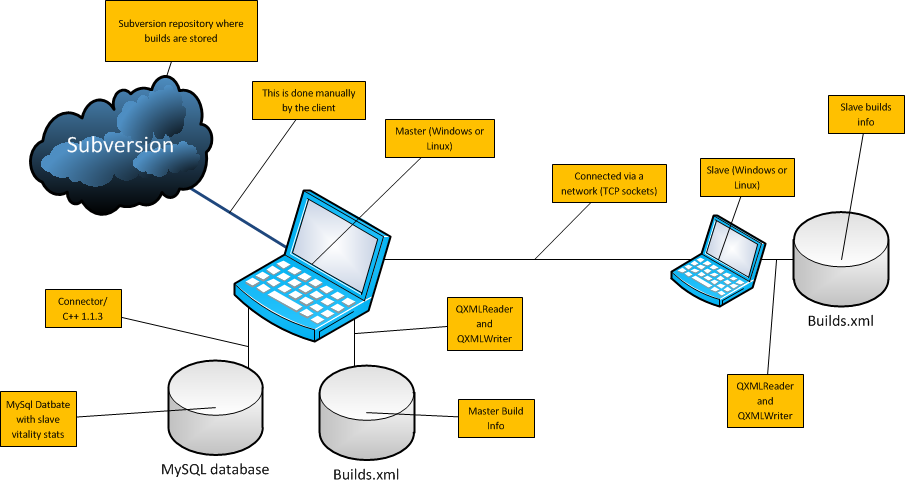
\includegraphics[angle = 90, scale=0.7]{ComponentDiag.png}
\end{center}








%\section{Technologies}

%\begin{itemize}

%\item{Platforms}
%\begin{itemize}
%\item{Windows}
%\item{Linux}
%\end{itemize}


%\item{Database}
%\begin{itemize}
%\item{XML based}
%\item{MySQL based}
%\end{itemize}


%\item{Network}
%\begin{itemize}
%\item{QT Framework Network API}
%\end{itemize}


%\item{Graphical User Interface}
%\begin{itemize}
%\item{QT Framework GUI API}
%\end{itemize}

%\end{itemize}
\newpage

\section{Glossary}
\begin{itemize}
\item{Build - An application build version that could potentially be distributed to slave computers.}
\item{Slave - A computer that will be controlled via a master computer. Application builds will be sent to this computer.}
\item{Master - A computer that will control Slaves across a network.}
\item{Server - A machine waiting on the network for connections from other machines.}
\item{GUI - Graphical User Interface with which a user can control the project.}
\item{Project - This project. The distributed application manager.}
\item{Application Configuration - Environment variables that are specified when running an application.}
\end{itemize}

\end{document}